\section{\textbf{Experimental Results}}
Table \ref{AE} represents accuracy and error rate of different classification algorithm on our dataset.
\renewcommand{\arraystretch}{1.5}
\begin{table}[h!]
\begin{center}
\caption{Evaluation Summary}
\begin{tabular}{|m{4.5cm} | m{1.6cm}| m{1.6cm}|}
\hline
     Classification Algorithm & Accuracy  & Error  \\
\hline
    Naive Bayes & 0.85 & 0.15\\
\hline 
    SVM (Linaer Kernel) & 0.91 & 0.09\\
\hline 
    SVM (RBF Kernel) & 0.90 & 0.10\\
\hline 
    Logistic Regression & 0.92 & 0.08\\
\hline
    K-Nearest Neighbor & 0.73 & 0.27\\
\hline
    Decision Tree & 0.88 & 0.12\\
\hline
\end{tabular}
\label{AE}
\end{center}
\end{table}
\par
Table \ref{prr} shows the precision, recall and $F_1$ score of different classification algorithm used in our model.

\begin{table}[h!]
\begin{center}
\caption{Performance Comparison}
\begin{tabular}{|m{3.6cm} | m{1.25cm}| m{1.2cm}| m{1.3cm}|}
\hline
     Classification Algorithm & Precision & Recall & $F_1$ score \\
\hline
    Naive Bayes & 0.89 & 0.85 & 0.85\\
\hline 
    SVM (Linaer Kernel) & 0.91 & 0.91 & 0.91\\
\hline 
    SVM (RBF Kernel) & 0.90 & 0.91 & 0.90\\
\hline 
    Logistic Regression & 0.91 & 0.93 & 0.93\\
\hline
    K-Nearest Neighbor & 0.82 & 0.73 & 0.70\\
\hline
    Decision Tree & 0.88 & 0.92 & 0.89\\
\hline
\end{tabular}
\label{prr}
\end{center}
\end{table}

For all of the algorithms we use similar number of training and test documents. From table \ref{AE} and \ref{prr}, we can see that Logistic Regression and Support Vector Machine algorithm's are performing up to the mark on our dataset. Naive Bayes and Decision tree also doing really well. But accuracy of K-nearest neighbour is really poor compare to other algorithms. 

Now, we will learn about classification report, Precision Recall curve and Receiver operating characteristic's (ROC) curve of  all of this algorithms. Classification report gives us precision, recall and $F_1$ score of each category which is really helpful to analyze the algorithm.
\subsection{\textbf{Naive Bayes Classifier}}
Table \ref{NBC} shows the classification report and \textbf{Fig.} \ref{prrn} shows Precision-Recall and ROC curve for Naive Bayes classifier.  .
\renewcommand{\arraystretch}{1.2}
\begin{table}[h!]
\begin{center}
\caption{Classification Report (Naive Bayes)}
\begin{tabular}{|m{2.8cm} | m{1.5cm}| m{1.3cm}| m{1.5cm}|}
\hline
     & Precision & Recall & $F_1$ score\\
\hline
     Suspicious & 1.00 & 0.71 & 0.83\\
\hline 
     Non suspicious  & 0.76 & 1.00 & 0.87\\
\hline 
     avg./total & 0.89 & 0.85 & 0.85\\
\hline
\end{tabular}
\label{NBC}
\end{center}
\end{table}

\begin{figure}[H]
\centering
\subcaptionbox{Precision Recall}{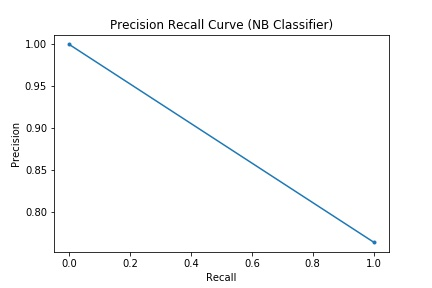
\includegraphics[scale=0.29]{Figures/PRN.jpg}}%
\hfill % <-- Seperation
\subcaptionbox{ROC}{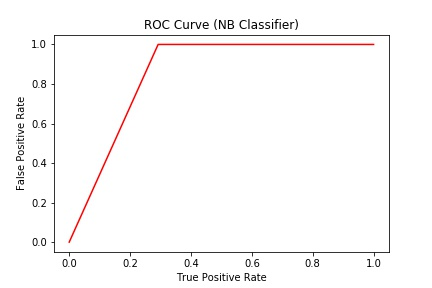
\includegraphics[scale =0.29]{Figures/ROCN.jpg}}%
\caption{Result of Naive Bayes Classifier}
\label{prrn}
\end{figure}


\subsection{\textbf{SVM (Linear Kernel)}}
Table \ref{SVML} shows the classification report and \textbf{Fig.} \ref{slk} shows Precision-Recall and ROC curve for Support Vector Machine with linear kernel.

\begin{table}[h!]
\begin{center}
\caption{Classification Report (SVM Linear Kernel)}
\begin{tabular}{|m{2.8cm} | m{1.5cm}| m{1.3cm}| m{1.5cm}|}
\hline
     & Precision & Recall & $F_1$ score\\
\hline
     Suspicious & 0.91 & 1.00 & 0.91\\
\hline 
     Non suspicious  & 1.00 & 0.90 & 0.91\\
\hline 
     avg./total & 0.91 & 0.91 & 0.91\\
\hline
\end{tabular}
\label{SVML}
\end{center}
\end{table}

\begin{figure}[H]
\centering
\subcaptionbox{Precision Recall}{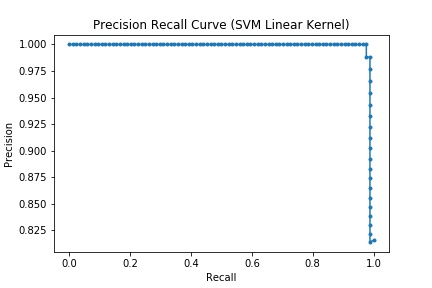
\includegraphics[scale=0.29]{Figures/PRSL.jpg}}%
\hfill % <-- Seperation
\subcaptionbox{ROC}{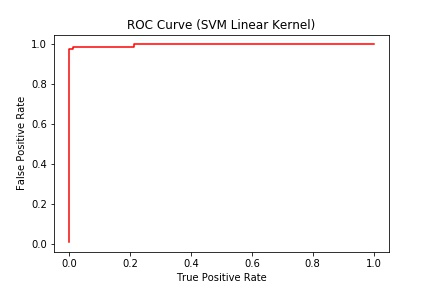
\includegraphics[scale =0.29]{Figures/ROCSL.jpg}}%
\caption{Result of SVM (Linear Kernel)}
\label{slk}
\end{figure}

\subsection{\textbf{SVM (RBF Kernel)}}
Results of Support Vector Machine with RBF kernel are shown in table \ref{SVMR} and \textbf{Fig.} \ref{svr}.
\renewcommand{\arraystretch}{1.1}
\begin{table}[h!]
\begin{center}
\caption{Classification Report (SVM RBF Kernel)}
\begin{tabular}{|m{2.8cm} | m{1.5cm}| m{1.3cm}| m{1.5cm}|}
\hline
     & Precision & Recall & $F_1$ score\\
\hline
     Suspicious & 0.90 & 0.99 & 0.90\\
\hline 
     Non suspicious  & 0.99 & 0.89 & 0.91\\
\hline 
     avg./total & 0.90 & 0.91 & 0.90\\
\hline
\end{tabular}
\label{SVMR}
\end{center}
\end{table}

\begin{figure}[H]
\centering
\subcaptionbox{Precision Recall}{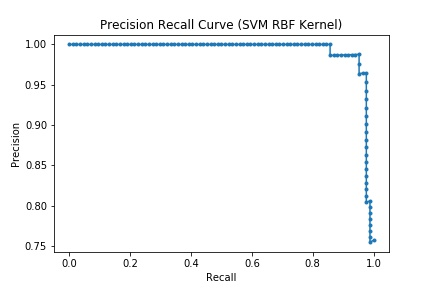
\includegraphics[scale=0.29]{Figures/PRSR.jpg}}%
\hfill % <-- Seperation
\subcaptionbox{ROC}{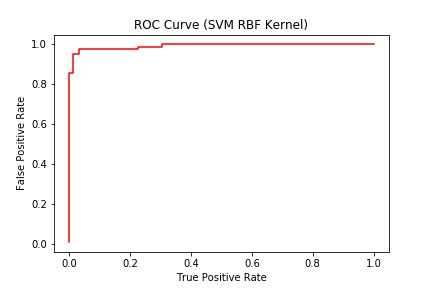
\includegraphics[scale =0.29]{Figures/ROCSR.jpg}}%
\caption{Result of SVM (RBF Kernel)}
\label{svr}
\end{figure}

\subsection{\textbf{Logistic Regression}}
Results of Logistic Regression classifier are shown in table \ref{lr} and \textbf{Fig.} \ref{flr}.

\begin{table}[h!]
\begin{center}
\caption{Classification Report (Logistic Regression)}
\begin{tabular}{|m{2.8cm} | m{1.5cm}| m{1.3cm}| m{1.5cm}|}
\hline
     & Precision & Recall & $F_1$ score\\
\hline
     Suspicious & 0.92 & 1.00 & 0.93\\
\hline 
     Non suspicious  & 1.00 & 0.93 & 0.93\\
\hline 
     avg./total & 0.91 & 0.93 & 0.93\\
\hline
\end{tabular}
\label{lr}
\end{center}
\end{table}

\begin{figure}[H]
\centering
\subcaptionbox{Precision Recall}{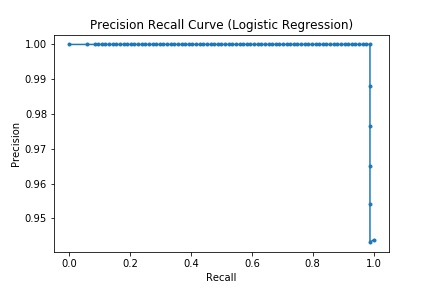
\includegraphics[scale=0.29]{Figures/PRLR.jpg}}%
\hfill % <-- Seperation
\subcaptionbox{ROC}{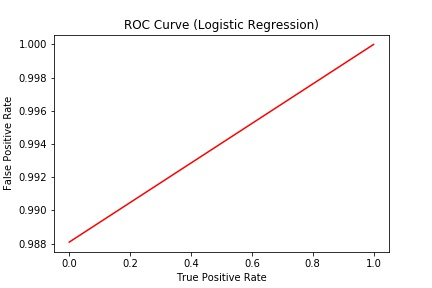
\includegraphics[scale =0.29]{Figures/ROCLR.jpg}}%
\caption{Result of Logistic Regression}
\label{flr}
\end{figure}



\subsection{\textbf{K-Nearest Neighbor}}
\renewcommand{\arraystretch}{1}
\begin{table}[h!]
\begin{center}
\caption{Classification Report (K-Nearest Neighbor)}
\begin{tabular}{|m{2.8cm} | m{1.5cm}| m{1.3cm}| m{1.5cm}|}
\hline
     & Precision & Recall & $F_1$ score\\
\hline
     Suspicious & 0.65 & 1.00 & 0.79\\
\hline 
     Non suspicious  & 1.00 & 0.44 & 0.61\\
\hline 
     avg./total & 0.82 & 0.73 & 0.70\\
\hline
\end{tabular}
\label{tknn}
\end{center}
\end{table}


\begin{figure}[H]
\centering
\subcaptionbox{Precision Recall}{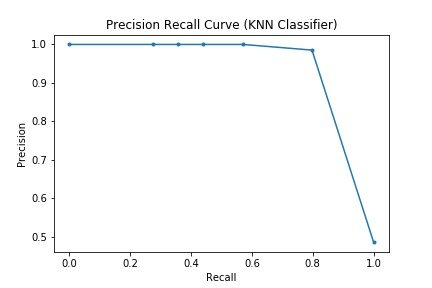
\includegraphics[scale=0.29]{Figures/PRKNN.jpg}}%
\hfill % <-- Seperation
\subcaptionbox{ROC}{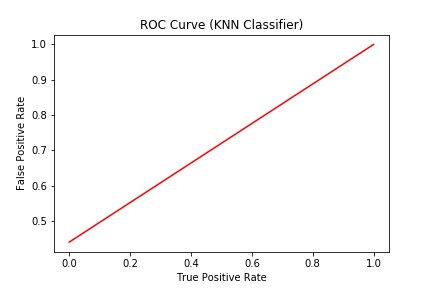
\includegraphics[scale =0.29]{Figures/ROCKNN.jpg}}%
\caption{Result of K-Nearest Neighbor}
\label{fknn}
\end{figure}

\subsection{\textbf{Decision Tree}}

Results of Decision Tree classifier are shown in table \ref{tdct} and \textbf{Fig.} \ref{fdct}.

\begin{table}[h!]
\begin{center}
\caption{Classification Report (Decision Tree)}
\begin{tabular}{|m{2.8cm} | m{1.5cm}| m{1.3cm}| m{1.5cm}|}
\hline
     & Precision & Recall & $F_1$ score\\
\hline
     Suspicious & 0.91 & 0.89 & 0.90\\
\hline 
     Non suspicious  & 0.88 & 0.90 & 0.89\\
\hline 
     avg./total & 0.90 & 0.90 & 0.90\\
\hline
\end{tabular}
\label{tdct}
\end{center}
\end{table}

\begin{figure}[H]
\centering
\subcaptionbox{Precision Recall}{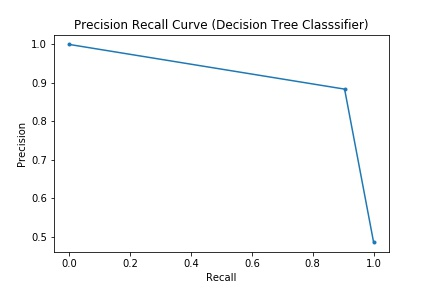
\includegraphics[scale=0.29]{Figures/PRDCT.jpg}}%
\hfill % <-- Seperation
\subcaptionbox{ROC}{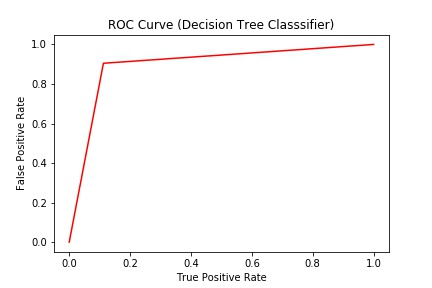
\includegraphics[scale =0.29]{Figures/ROCDCT.jpg}}%
\caption{Result of Decision Tree}
\label{fdct}
\end{figure}
